\documentclass[english]{tktltiki}
\usepackage[pdftex]{graphicx}
\usepackage{subfigure}
\usepackage{booktabs}
\usepackage{url}
\usepackage{amsthm,amssymb}
\usepackage{amsmath}
\usepackage{todonotes}
\usepackage{comment}

\begin{document}
\onehalfspacing

\title{Interactive Office Project}
\author{Jan Lippert, Michael Morasch, P\'eter Ivanics}
\date{\today}

\maketitle

\numberofpagesinformation{\numberofpages\ pages + \numberofappendixpages\ appendices}

\begin{abstract}
Break habits are essential part of everyday work life. They help us to refresh our brain, renew mentally and physically by putting work-related thoughts and activities apart. Undoubtedly, regular break habits lead to better efficiency of workers, independently from workplace and business area.

The goal of our research is to suggest development possibilities to any office environment. Through literature review, observation and semi structured interviews we identified that regular break habits lead to more effective work and also create a better atmosphere. As a result, relationships between co-workers develop, inhibitions disappear and work-culture gets better. However, some employees may not take breaks regularly or have strong relationships with their colleagues. 

In this study, we identified the need for a tool that helps individuals to take breaks more regularly in a fun and interactive way. We then developed a software solution for this purpose. The software aims to improve regularity of breaks taken in any office environment by matching random colleagues with similar interests and professional background for spending breaks together. 

The core functionality of the software was designed and a prototype was implemented by the end of the project. The software is ready to be tested in a real environment with real users, however the actual evaluation was not yet covered until the publication of this paper. However, the expert evaluation on the user interface of the software has identified room for improvements and could be interesting topic of further research. 
\end{abstract}

\mytableofcontents

\section{Introduction}
The goal of our project is to improve the office by utilizing smart and interactive technologies. This report will investigate different areas of interest in that goal. 

One area of interest is to improve the efficiency of employees and the office itself which is investigated in section \ref{sec:efficiency}. Better collaboration is a very important part of efficiency and will be investigated in section \ref{sec:collaboration}. Section \ref{sec:comfort} will take a at how a comfortable and enjoyable working environment can increase the productivity and creativity of workers. Finally, \ref{sec:safety} reports shortly on how modern technologies can be make the working environment safer.

\section{Background and motivation}
% the context in which the course was started
During the course lectures, several areas of Human-Computer Interaction (HCI) and related areas were presented and discussed. The course material covered several aspects of research in this area, such as user research, needfinding, prototyping methods and product evaluation. Furthermore, popular areas of research, such as augmented and virtual reality, ubiquitous computing, physiological computing were discussed. 

% what were the original ideas and how the interactive office came to surface?
The topic of Smart Home applications was one of the possible research areas to dive into, which served as the origin of the present research. Despite the fact that the technology in such application field is studied for a long time already, the solutions are yet limited to the home/living environment. By living environment we mean a setting, where people live either on their own or in a family, perform household-related activities (e.g. cooking, cleaning), spend their free time together and so on. At the same time, Smart Home solutions bring household maintenance to a new level by introducing interactive, computer-facilitated solutions to enhance energy-efficiency and well-being of families. 

% how does our idea differ, what are the main similarities and differences? 
At the first place our group started thinking, how such solutions could be utilized in a different setting, such as an office or a working environment. Starting from existing Smart Home solutions we could derive several aspects that could be brought into a Smart Office solution, such as: 

\begin{itemize}
	\item energy-efficiency, 
	\item automation of recurring tasks,
	\item well-being of employees in the office,
	\item enhancement of work culture and atmosphere, 
	\item workforce management, workload tracking and optimization,
	\item efficient maintenance of electronic devices and facilities.
\end{itemize}

% why is this research area important? 
Undoubtedly, the above aspects are relevant in numerous places and settings. For example, companies that operate in any field of industry are likely to have an office, where the employees do their everyday job. Naturally, it is in the interest of the corporation to address the aspects listed above to enhance efficiency, quality work and atmosphere. 

\section{Needfinding}
\subsection{Stakeholder analysis}

% under what circumstances the analysis was carried out?
The needfinding began by analyzing the stakeholders of the research. We started to think from the point of view of an IT office environment, because this is an area where our team members had personal experience and interest. However, we did not limit our analysis and extended to other fields, for example banking, law and libraries. 

\todo{We should redraw this in Visio or similar software - Peter}
	\begin{figure}[h] 
		\begin{center}
			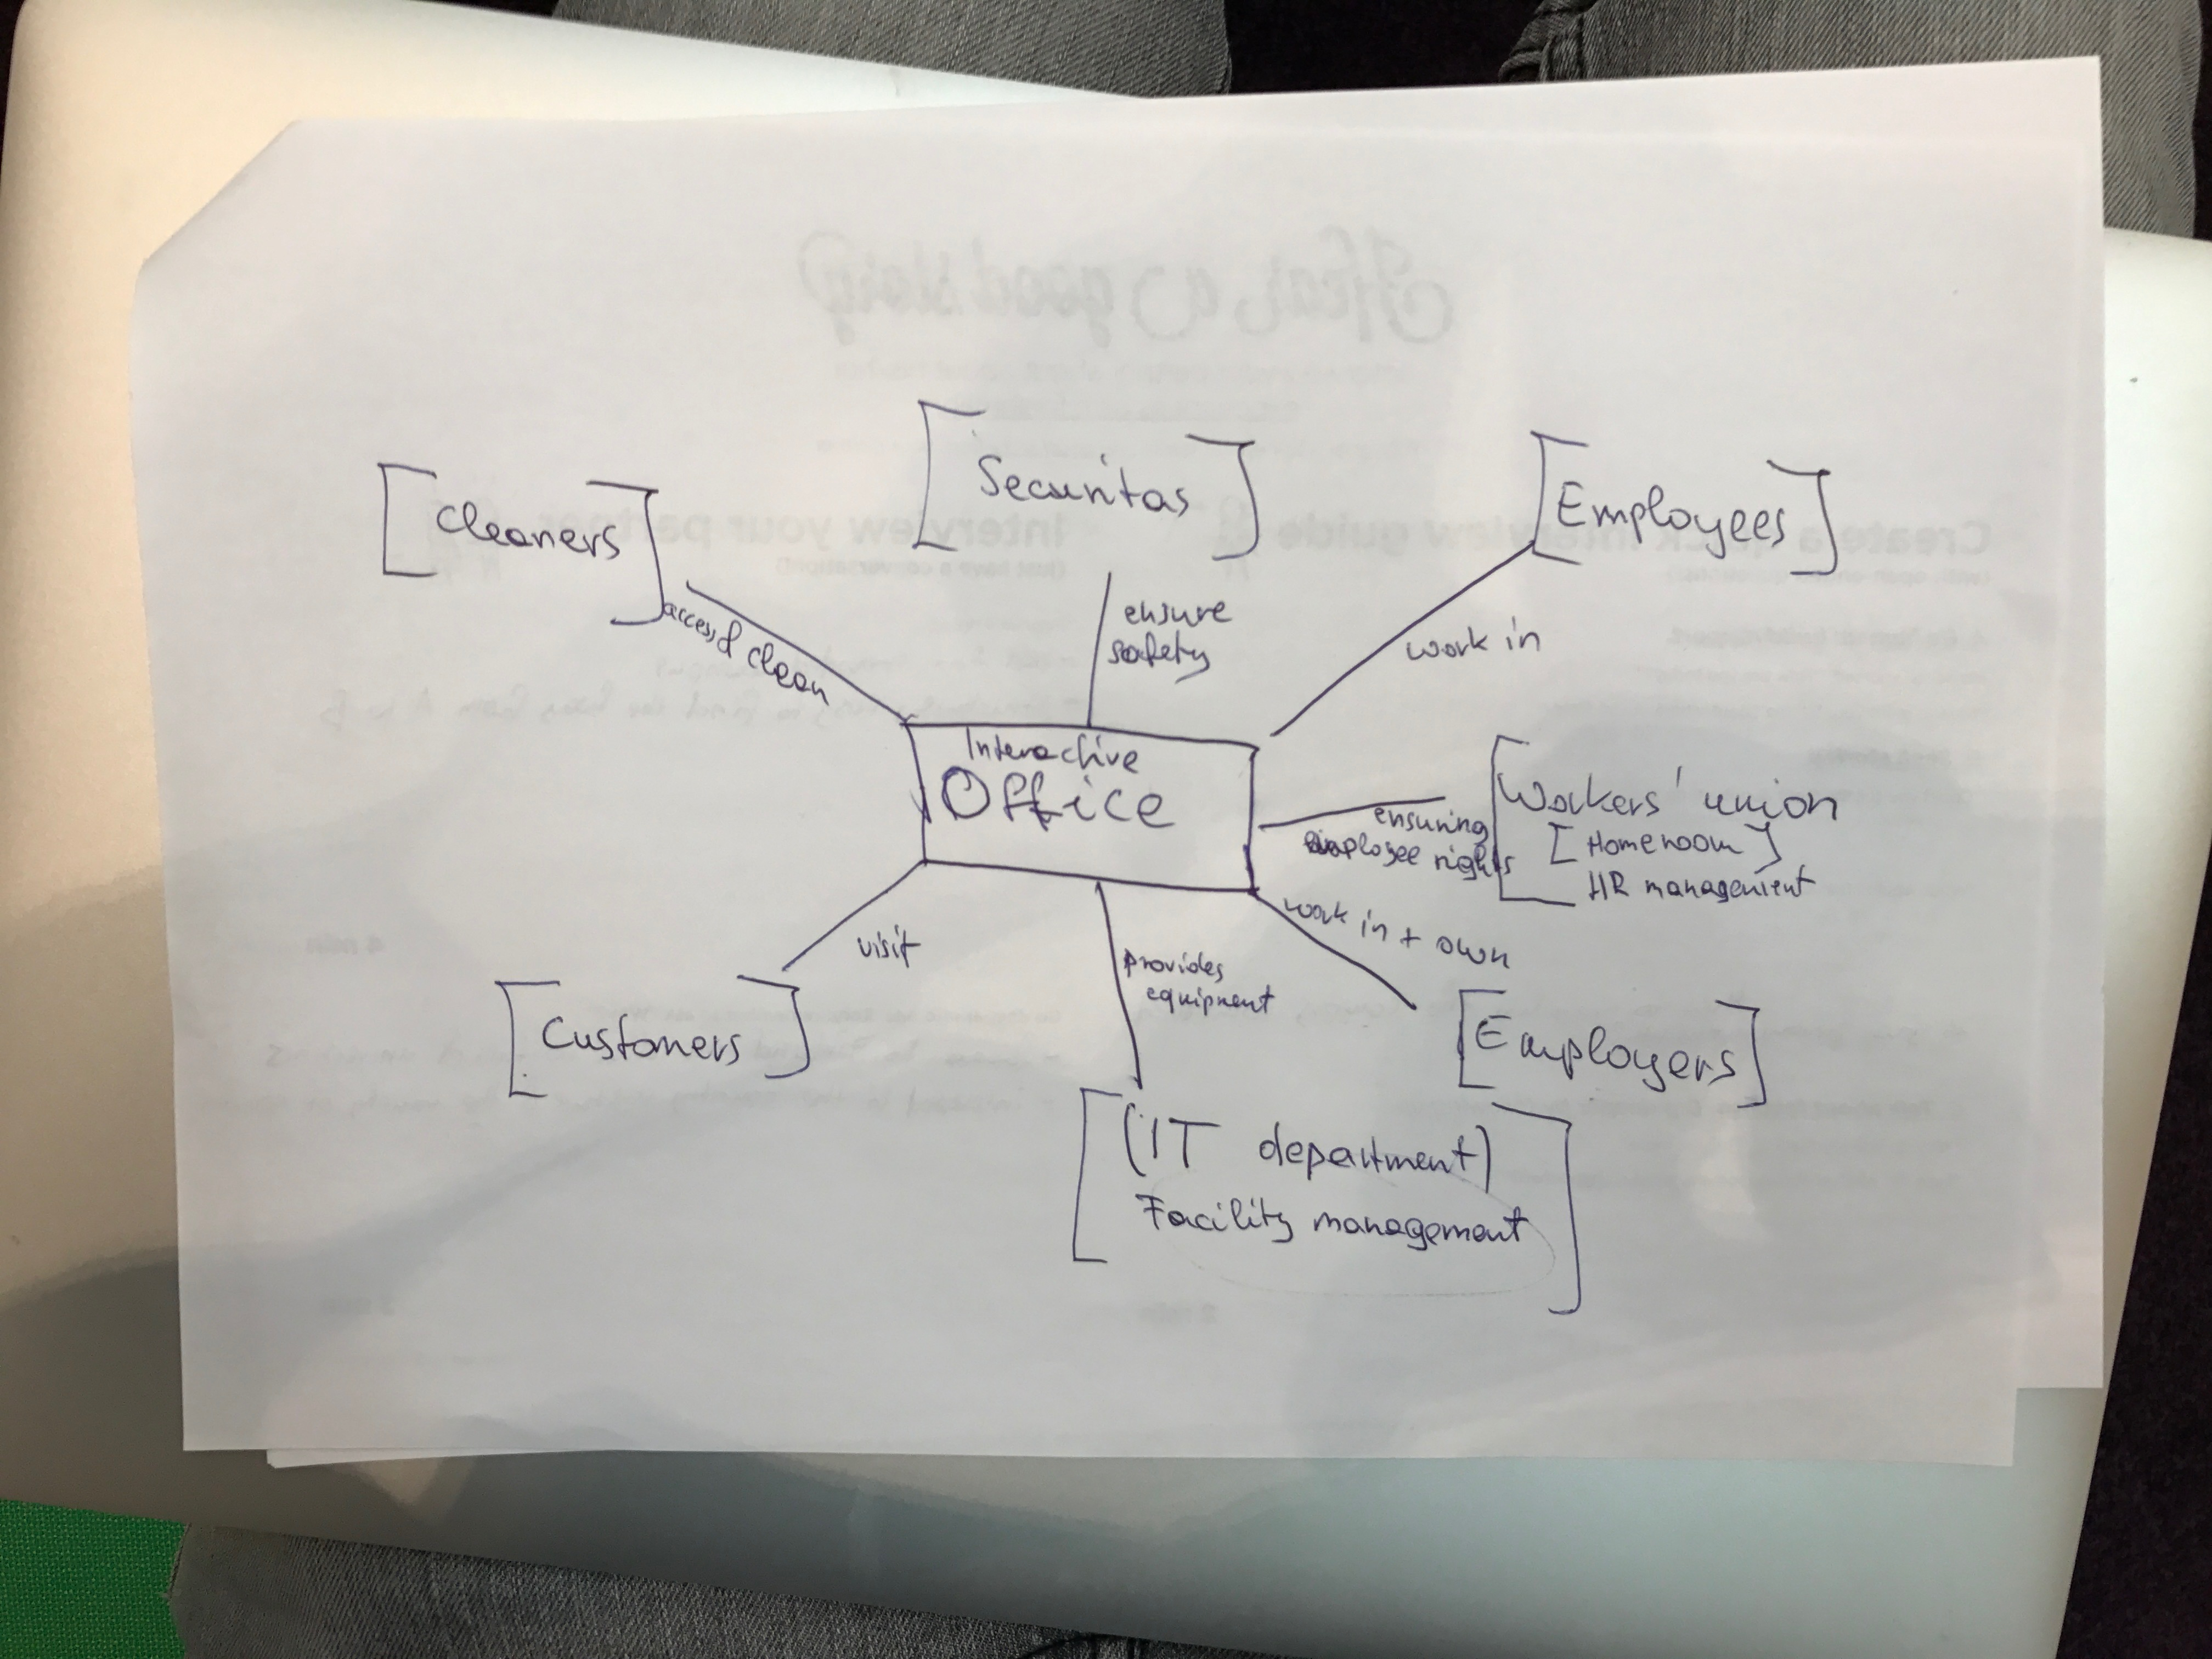
\includegraphics[width=0.9\textwidth]{images/stakeholdermap.jpg}
			\caption{The stakeholder map in an office environment.}
			\label{stakeholder_map}
		\end{center}
	\end{figure}

% who are the stakeholders? 
During our analysis, the following stakeholders were identified. The stakeholder map is displayed on Figure \ref{stakeholder_map}. 
\begin{enumerate}
	\item Employees
	\item Employers
	\item Customers/Visitors
%Potential and existing customers of the firm
%Business partners, investors
%Third parties, e.g. bank representatives, TEKES, …
%Relatives of employees
%Come to visit the office occasionally
%Stay for a short while
%Meetings, Coffee
%Initial information on the structure of the office
%Where to find the meeting room/person (s)he came to meet
%aula to wait for the person if busy
%(AI receptionist?)
	\item Cleaners
%Somebody who is cleaning the office
%One or more
%Once a day/week, …
%(AI cleaning robots)
%Optimal path to clean the office
%(sensors to check consumables?)
%(buttons in every room (green/red) which employees can press to “order” cleaning service) -> mobile app for employees
%Lights on when cleaning starts -> lights off in the room when the cleaning is complete and tables green/red indicators
%Number of ordered cleaners corresponds to the rooms marked as to be cleaned
%(Indoor Navigation?)

	\item IT Department
%People responsible for the maintenance of the (IT) infrastructure of the office
%Their goal is to ensure the functionality of the electronics in the office (e.g. lights, air conditioning, heating, …)
%Sensors to expensive devices to indicate if they’re wearing or not -> in case an error occurs, IT department should be notified where the device is and what the problem is
%Tablet can help to find the way to the device
%(Indoor Navigation?)
%Expensive/Valuable devices should stay in the office

\end{enumerate}

% what are the connections between the stakeholders? 
The stakeholders are connected through the office environment with slightly different needs. For example, a regular employee in the office experiences different means and performs other kinds of tasks than a cleaning lady. Nevertheless, a common purpose is the efficient and precise completion of work-related activities for all parties. Individuals may interact with one another and have to perform tasks collaboratively, together. The infrastructure that is provided by the office may be shared and used by multiple parties. 

Therefore, we concluded that the collaboration, interaction and the proper facilities in the office are essential aspects to carry on with the research. On top of that, the environment has to facilitate efficient work as well as quality outcome of all parties. As a future vision, we imagined an interactive office environment that facilitates all the aspects and needs covered by the stakeholders above. 

% what was excluded?
On top of the stakeholders listed above and displayed on Figure \ref{stakeholder_map}, other parties were identified. For instance, we were thinking of how the Worker's Union or security companies may benefit from a more interactive office environment, however we concluded that such analysis is out of the scope of our research. Therefore, our focus was moved towards other directions. 

\subsection{Social Data Analysis}
Since the goal of our project is to solve an existing need, a social data analysis was conducted to 
identify potential areas of improvement. Multiple blogs and other internet sources were investigated 
and compared with each other to identify common patterns and areas of interest for the smart or 
interactive office. This section will outline the four key-areas that were identified in the social 
data analysis.

\paragraph{Efficiency}\label{sec:sda-efficiency}
Improving the efficiency of workers is one of the key drivers of change in workplace strategies 
according to \cite{hub13}. A smart or interactive office can help with this goal. Tools and software 
can help to reduce the time employees spend on tasks that are not directly related to profitable 
goals of the company.

Both \cite{iotagenda} and \cite{roomzilla9} describe that managing rooms is a tedious task. 
Roomzilla -- a software company selling room booking software -- estimates in \cite{roomzilla9} how 
much cost managing rooms without software can cause. The authors assume that office manager managing 
room bookings spends around 90 minutes per day to do so. Based on the average salary of an office 
manager in the US (\(20,65\text{USD}\)) the final estimate of this task is around \(681,45\text{USD}\) 
per month. The authors also mention some problems that can cause hidden costs: both late running 
meetings and overbooked rooms prevent employees from using their time to do actual work. 

The authors of this article instead describe how tracking room usage can lead to a better use of 
time. They propose a system that tracks room usage and makes the data available via Outlook or an 
appropriate alternative. This also helps employees to find a room when needed and therefore leads to 
less distractions and waste of time \cite{iotagenda}.

The tracked usage patterns can be utilized to save time and also to conserve energy. A smart or 
interactive office can turn on lights and devices in advance. In turn, the lights and devices can 
also be switched off when they are not needed anymore \cite{hbcommunications}.


\cite{hbcommunications} also outlines how AI and machine learning could be used to save employee 
time. They use the example of a smart call system with an automated menu that learns to direct calls 
to the correct department. This will reduce the time that is spent on redirecting callers and 
therefore improve the employees' efficiency. However, machine learning could also be used to suggest 
the best meetings times or predict when rooms are available.

Some other causes of wasted time in companies are technical problems in \cite{roomzilla3}. 
Especially in meetings these problems can take up some time. Sub-optimal setups, used (but not 
booked) rooms, and technical failures can cause delay of the meeting start and as such potentially 
lead to long-running meetings. The authors of \cite{roomzilla3} propose streamlined processes to 
make meetings more efficient. 

\paragraph{Collaboration}\label{sec:sda-collaboration}
Another key factor for innovation in the office outlined by \cite{hub13} is the hunt for and 
utilization of talented people. One major factor of keeping employees happy is to support different 
styles of work. This includes silent working areas to focus on projects, rooms to receive phone 
calls, but also areas where ``the atmosphere is conducive to innovation'' \cite{tieto}.

If these areas are provided, the employees must be able to freely move between these areas. One 
solution for this are non-fixed working desk, i.e. employees pick their working place when after 
they arrive in the office. \cite{occupiee}.  also outlines that flexible offices are needed as more 
employees work mobile and may rarely return to the office. In a flexible office environment with 
shared desks, the smart and interactive office must provide ways to find out where space is 
available and where colleagues are currently working \cite{tieto}.

Such technologies can be also be utilized to improve working together. If a project requires 
specialists, spontaneous meetings can be held by seeing who's currently available, where they are 
and what meeting room can be used \cite{tieto}. Similar results are mentioned \cite{hbcommunications} 
where the authors describe how streamlined communication and improved connectivity leads to better 
and faster collaboration between organization experts \footnote{\cite{hbcommunications} also 
mentions how automation of heating and lighting can lead to a more ``fun'' office improving the 
well-being of employees.}.

The importance of exciting workplaces for the creativity of employees is also mentioned in 
\cite{roomzilla3}. While typically it is assumed that such a playful environment may be detrimental 
to the productivity of employees, such environments can actually lead to a more creative and 
productive employees \cite{metroffice}. This in turn leads to better results and therefore a more 
successful business.



\paragraph{Comfort}\label{sec:sda-comfort}
Modern LEDs provide great ways to improve the worker's productivity by adapting intensity and the 
color spectrum. It has been shown in recent research that the color spectrum directly influences the 
activity and biorhythms of people  \cite{living-lab}. \cite{iotagenda} also highlights, how smart 
lighting can be used to create a more comfortable working environment.

Another important factor of well-being is acoustics. Most open area offices are too quiet and as 
such talks between colleagues and phone calls distract other people. However, too loud environments 
are also detrimental to work. Therefore the right balance as to be found \cite{living-lab}. 

Another possibility of the smart and interactive office is the automatic regulation of room 
temperature based on the time of day. Both \cite{iotagenda} and \cite{living-lab} outline the 
importance of temperature in the well-being of employees. People expect good thermal regulation in 
the office and it is also necessary to focus on work. But not everybody does feel temperature the 
same way. The living lab therefore developed and currently a ``climatic chair'' that helps each 
individual to regulate his or her working surrounding temperature \cite{living-lab}.


\paragraph{Safety}\label{sec:sda-safety}
Industrial workplaces like factories can be dangerous. While this is not directly related to a smart 
or interactive office, it is nonetheless an important factor in a smart workplace. \cite{sda-wired} 
lists a deadly accident which could possible have been prevented by utilizing modern technology.

In January 2012, one worker of the ArcelorMittal Burns Harbor steel-mill died while investigating 
noise in an oxygen furnace. The cause of death was a bursting pipe that released hot steam. The 
burst was caused by previously built-up pressure. A smart workplace could have prevented this 
accident by tracking pressure data in the pipe and warning workers to keep clear of the dangerous 
area.

Possible implementations of such a system could use apps, mobile devices, and wearables. In case of 
danger, acoustic and visual notifications could be send to the user. While such devices are widely 
available, \cite{sda-wired} mentions that software is lacking behind. The software of such systems 
must be intuitive to use. Also, the whole office and workplace has to be integrated: IT, machines, 
sensors, and finally the workers' devices. Since sensors produce a lot of data, \cite{sda-wired} 
also mentions that improved algorithms for streamed data analysis are needed.

\paragraph{Results}
The social data analysis verified, that a smart and interactive office can help to improve the 
efficiency of employees in various ways. One need that many of the papers outlined was the 
well-being of individuals because comfortable employees will produce better results.

Another important area was collaboration. This area can be improved by providing flexible working 
environments and better ways of communication. While some tools exist in this area, there is still 
way for improvement. 

Another final point which was identified is missing automation: much time is wasted by employees 
doing things manually that could be supported well by tools. Many of these tasks may be repetitive 
and also prevent the employee from doing ``actual work'' -- which in turn provides the chance to 
remove or simplify these automatable tasks.


\subsection{Observation}
To gain more understanding on the needs, an observation was carried out by the researchers. The reason for choosing this way of data collection is mainly triangulation, which provided us knowledge on the investigated domain from a different angle. On top of that, one of the team members works in an IT office environment in Helsinki, which allowed us to live with this possibility. For sake of confidentiality, the name of the firm and the exact details remain hidden in this report. 

The observation is carried out on a regular workday in the office when most of the employees are present. The room in which the observation is done is shared with four other colleagues. The observed environment is in between a corridor and another room in which other people are working. Therefore, there are multiple people actively working in the room, while occasionally others pass through. Accordingly, the environment is fairly noisy in general and there is some movement and interaction between employees. The room is equipped with rising desks and a whiteboard, that is used for work often by the employees. 

The observed insights and their short descriptions are, as follows:

\begin{enumerate}
	\item \textbf{Arrival to the office}: the first employees started to come around 9 AM and began to work in piece. As more and more people arrived to the office, the level of noise, interaction and movement increased naturally. Typically newcomers greeted their colleagues and initiated casual conversations with fellow coworkers (e.g. by asking how are you today, how was last afternoon, did you get stuck in the traffic as well?). However, some workers just entered the room with a coffee, sat down and began to work. 
	\item \textbf{Meetings}: around 10 AM, some colleagues left for a regular Daily Scrum meeting, which was hosted in another room. Throughout the working days, there are many prescheduled and recurring meetings, which are always hosted in one of the meeting rooms. Others left to their own private meetings/Skype calls during the day so that others are not disturbed and remain focused. In some cases however, people had ad-hoc face-to-face meetings or phone calls in the room which increased the level of noise and disturbance towards others.
	\item \textbf{Noise and interruption}: noise tended to be disturbing in some situations to employees. In most cases once somebody entered the room, he or she began to talk to one of their colleagues which dragged the attention of other workers in the zone. The disturbed employees either joined the conversation (which was either casual or work-related) and changed their attention from their computers to the person who just entered the room. This may or may not be a problem as these interruptions can be constructive to employee relationships or knowledge sharing in the company, but some may consider them as unnecessary interruptions. 	
	\item \textbf{Light in the room}: one interesting observation made during the day was pointed out by one of the employees in the office. Namely, the room has only one window and there is no natural light source coming in from the street. This fact is annoying for employees who work in this room for a long time as days are very short during the Finnish winter and there is not too much natural light whatsoever. For this reason, the company installed a device (similar to the one displayed on Figure \ref{artificial_sunlight}) that provides artificial sunlight that is turned on most of the day. 
	
	\begin{figure}[h] 
		\begin{center}
			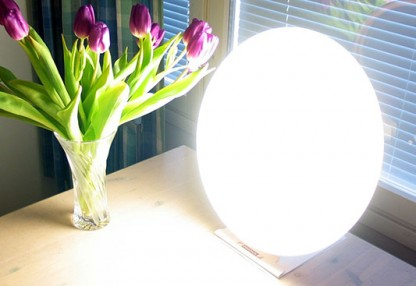
\includegraphics[width=0.9\textwidth]{images/artificial_sunlight.jpg}
			\caption{The office is equipped with a device that provides artificial light to the room with weak access to natural sunlight (the picture is only an illustration).}
			\label{artificial_sunlight}
		\end{center}
	\end{figure}
	\item \textbf{Interaction and breaks}: despite the morning chit-chat and the meetings, colleagues did not interact too much. Mostly, people were into their computers and their work, some even so much that seemingly they did not take any break despite lunch. 
	\pagebreak
	\item \textbf{Cleaning service}: at the end of the day, the cleaners arrived to the office. Their duties during workdays seemed to be limited to gather all glasses and cutlery from the desks of the employees and bring them to the common kitchen on the floor. Seemingly, the only cleaning lady had to make several rounds between the kitchen and the different rooms as the employees left many dishes all around the office. This seemed to be time consuming and probably would have been much faster if the items would be in the kitchen already. 
\end{enumerate}

\subsection{Interviews}
% what kind of interviews were conducted and why? 
To gain further understanding on the needs and the opinions of the stakeholders, we decided to conduct semi-structured interviews. The reason behind choosing this method of data collection is that it provides fairly large amount of quantitative data in a short time and on low cost. We also realized that through our networks we can reach stakeholders with different background and interest and therefore easily collect data from different business areas. 

The interview questions (Appendix \ref{sec:interview-questions}) were designed together with the student tutors in one of the exercise sessions. The interviews were conducted on the upcoming weeks before the prototyping began. The transcripts of the interviews are displayed as appendices to this document. In overall five interviews were conducted with interviewees from slightly different background. During the interview phase we put some focus on the diversity of the participants so we also learn more about the problems and habits in various environments. The analysis of the findings was performed once the interviews were conducted together in a session together with the tutors.

The interviews highlighted that most of the interviewees think about themselves as they take breaks regularly. Breaks are often spent together with other colleagues, but some interviewees like to relax on their own. During the breaks interviewees do not seem to talk about work-related issues, unless necessary. This allows us to conclude that the breaks are more about relaxation, refreshing the brains and returning to work with a clear mind once they are over. 

Despite the fact that some spend breaks with colleagues, many colleagues do not know hobbies and personal background of one another. We conclude this by often hearing that colleagues tend to know what others do in their work, but not their hobbies. The reason behind this may be that private life is a personal topic and some may not like to talk about it in a working environment (as pointed out by the librarian at University of Helsinki [see transcript in the appendix]). 

Interestingly, there was an agreement among the interviewees that the good work atmosphere leads to better collaboration in the environment. This means if colleagues enjoy their time and are comfortable to work with co-workers, the interaction between them and hence the success of their collaboration increases. 

\subsection{Crowdboard}
\label{sec:crowdboard}
We were offered to use the Crowdboard to help with  need-finding and ideation. The Crowdboard is an augmented white-board, designed and developed at the Helsinki University. The Crowdboard consists of multiple screens whose content is shared online with workers from Amazon Turk\todo{Add link? -- jan}. This enables the Amazon Turk workers to see the notes on the white-board and to post comments on these notes. Figure \ref{fig:crowdboard-diagram} shows a diagram of how the Crowdboard works \cite{crowdboard}. 

\begin{figure}[h]
 \centering
 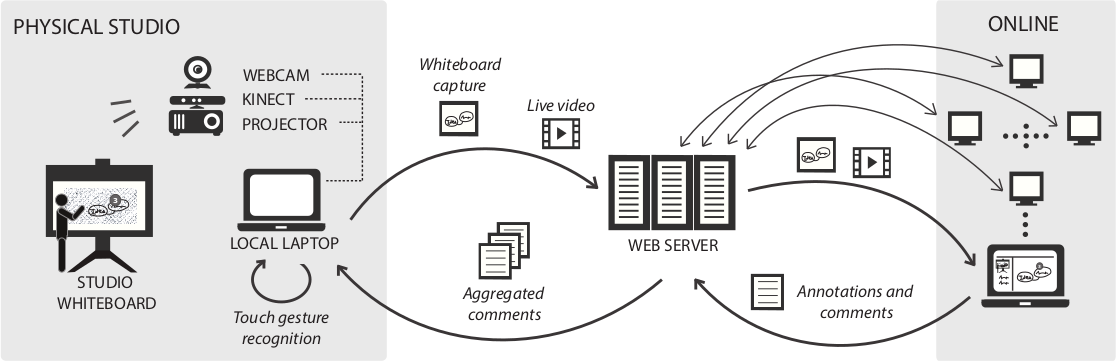
\includegraphics[width=\textwidth]{images/crowdboard-diagram.png}
 \caption{Overview over the Crowdboard's architecture \& information flow \cite{crowdboard}}
 \label{fig:crowdboard-diagram}
\end{figure}




In the Crowdboard session our team had three loosely related goals: we wanted to find out what people are doing in their break-time and what motivates them to take a break. We also wanted to validate our ideas and see if people would be willing to use our system. The final goal was to find out new ideas by pitching rough drafts and gathering ideas. Before doing so, the Amazon Turk workers had to be invited(Appendix 3) \todo{note that actual invitation was slightly different?}.

Furthermore, we had to prepare an initial task to Turkers joining the Crowdboard session (Appendix 4).

The experiment took place on the afternoon of March 23, 2017. There were ca. 20 Amazon Turk workers participating in the session. We got around 40 useful comments on the ideas that were discussed. As mentioned before, we had three goals in this session.

The first goal was to find out what people do in their breaks. As we suspected, many people eat something in their break. There were some suggestions on how to make the lunch break more interesting: 3 people suggested having lunch or ordering food together with everyone in the department or, if a kitchen is available, to cook together\todo{First one is common in my company at home. Note? -- jan}. Other results of the Crowdboard session include: 
\begin{description}
  \item[Coffee Break] We suspected that coffee breaks are a common break activity. This was verified in multiple interviews and also in this Crowdboard session.
  \item[Board Games] We had the idea for our application to suggest board games as one acitivity to bring colleagues together This suggestion was repeated in the Crowdboard session while another comment suggested to do puzzles or crosswords.
  \item[Waling/Outside breaks] Another suggestion from the session that could be added as an activity in our application.
\end{description}


\begin{comment}
Break Habits
\begin{itemize}
  \item \textsl{Snacking, Lunch, Overeating, Conferences with food}
  \item \textsl{Smoking}
  \item Procrastinating
  \item Reading
  \item Texting
  \item \textsl{Puzzles, Crosswords}
  \item \textsl{Board games, chess or checkers}
  \item \textsl{Go outside, walking break}
  \item Personal or resting break
\end{itemize}
\end{comment}

Since our team consists solely of non-smokers, we did not think of smoking breaks. This was an activity discovered by the Crowdboard session. However, the discussion was primarily focussed on the potential health damages. So while smoking is a valid break activity, we will not encourage smoking with our application and suggest other activities instead.\todo{is interesting, but could be removed without ``damage'' -- jan}

Some time into the session, we introduced the idea of suggesting more active breaks, e.g. sports. This idea also attracted some comments including ``people who share a common activity probably develop
connections faster''.

\begin{comment}
would you like to do "active" breaks? sports etc
\begin{itemize}
  \item Setting up a small game table such as table tennis and
holding tournaments
  \item Take walks around the building
  \item stretching
  \item people who share a common activity probably develop
connections faster
\end{itemize}

suggestion of colleagues to take breaks with?
\begin{itemize}
  \item use time to connect with someone new
\end{itemize}
\end{comment}

\begin{comment}
tournaments \& leaderboards
\begin{itemize}
  \item A break room
with games, vending machines, tounament equipment etc
  \item Having on going health bets or competitions
a raffle with reward incentives
  \item free coffee, barnes and nobles gift certificate
  \item You could have people who are partnered up with the
desktop app work together to solve a puzzle for
competition or leaderboards
  \item Jeopardy game using work information
exercise room with interactive gaming like example Wii
  \item Healthy competition will increase happiness too and coherence
\end{itemize}
\end{comment}

The second goal of the Crowdboard session was to find out when or why people take breaks. We were looking for triggers that do not necessarily relate to lunch breaks. The comments on this topic were mostly related to stress, fatigue, or ``getting stuck''. There were only a few comments on this topic.

\begin{comment}
triggers break
\begin{itemize}
  \item When I hit a wall on a project
  \item stress, fatigue, work pressure
  \item not delegating tasks well
  \item no work available
\end{itemize}
\end{comment}


The final goal was to find out if people would use a system that suggests them to take a break with another person and also suggests some activities. The idea to match up different people received positive or neutral comments; one could use the break to ``connect with someone new''. It was also mentioned that ``set breaks would help people take the breaks together''.


We also mentioned the idea of using a ``pressure chair'' to determine how long a user has been working. There was only one useful comment on this idea which suggested to use pressure sensors on the keyboard instead.

All in all, many of our ideas and assumptions were verified in the Crowdboard session. We also got many new insights and were also notified of some things we missed.

\begin{comment}
technology
\begin{itemize}
  \item using an app to coordinate with workers through phones
or computers to alert unannounced breaks
  \item Video games
  \item There could be a desktop app that lets them know they
need to take a break soon based on when they clocked in
for work.
\end{itemize}

set breaks after specific time - 
\begin{itemize}
  \item Set breaks would help people take the breaks together.
\end{itemize}

pressure sensor chair
\begin{itemize}
  \item There should be pressure sensors on the keyboard. It can
identify issues with carpal tunnel
  \item Go green and healthy, it will promote a positive
environment
  \item Yoga room or a work gym where associates can socialize	
  \item An employee lounge will be nice, with a tv, healthy snacks,
using green materials
\end{itemize}
\end{comment}



\section{Development}
\label{sec:development}
This section describes the development phase of our project. The development was started around the end of the needfinding phase once the team had a clear vision on the problems we were about to address and the solutions to get over those.

\subsection{Proposal}
% what do we propose? 

% what are the scenarios in which the solution can work? 

\subsection{Project planning and tooling}
Right before jumping into the development, the roles of the team members were chosen, the available resources were considered and our availability was analyzed. We discussed how individuals can contribute to the final outcome of the project, how we can use our tutors' resources, what the main milestones in the project are and how much time can the team members dedicate to this project. 

The Gantt chart on Figure \ref{gantt-chart} summarizes the project's timeline, with the main milestones and activities. The purple lines mark the scheduled time for the activity, while the orange lines mark the time frame in which an activity was executed, but not originally planned.
 
\begin{figure}[h] 
		\begin{center}
			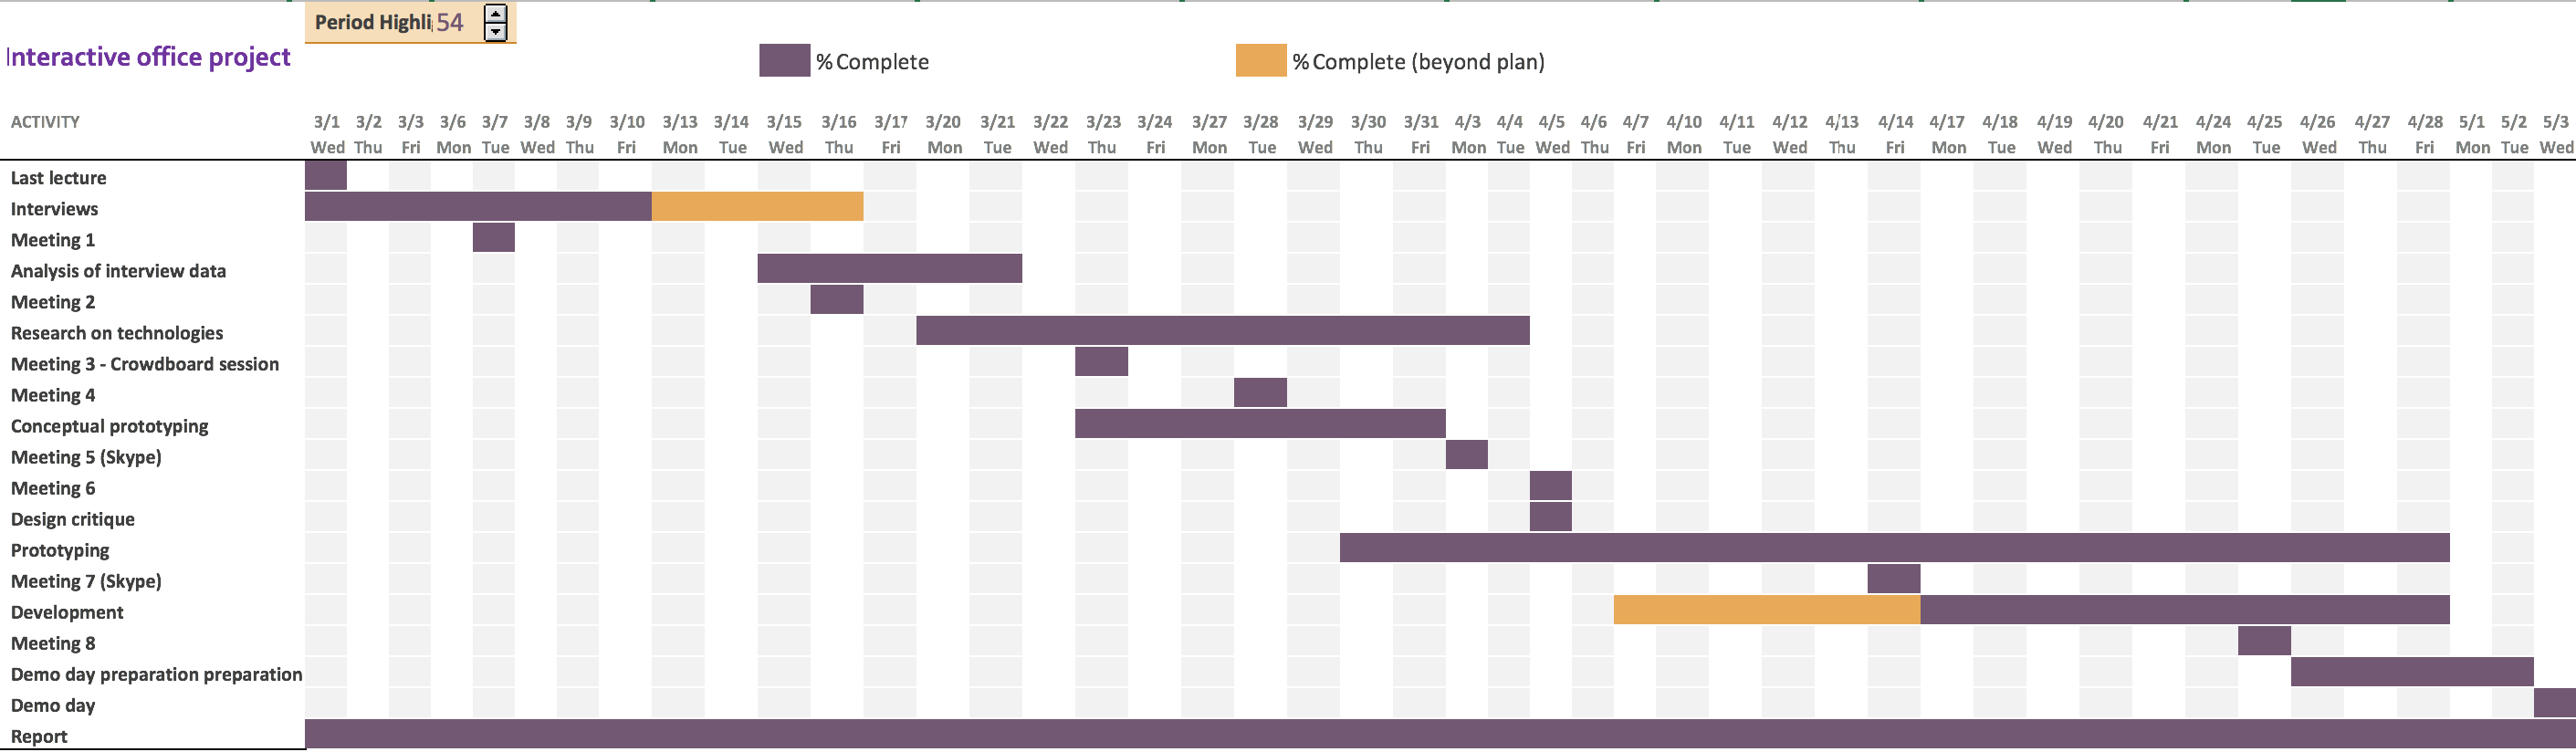
\includegraphics[width=1\textwidth]{images/gantt-chart.png}
			\caption{The Gantt chart of the project.}
			\label{gantt-chart}
		\end{center}
	\end{figure} 
 
% github as a working tool
To make the communication and knowledge sharing among team members, a Facebook group and a Google Drive folder was configured. For future source code version tracking, a Github page\footnote{\url{https://github.com/orgs/InteractiveOfficeProject/}} was configured. The full source code of the project and the report is made available through this page for the public. 

For the wireframes and prototype design, Microsoft Visio was used. To design the APIs, a Swagger \footnote{\url{http://swagger.io}} page was modified. Xamarin IDE \footnote{\url{https://www.xamarin.com/}} (Integrated Developer Environment) was used for the client's development.

\subsection{Chosen technologies}
The application is separated into a client and a server application.
% what resources are utilized for carrying the project out? 

% what technologies, development principles are chosen and followed and why? 

%what do we build upon?

\paragraph{Client} It was decided to develop the client in GTK\#. We chose this framework because it is platform-independent -- our client will be able to run on Linux, MacOS, and Windows -- and we were familiar with C\#. We decided to create a minimum viable product (MVP) and extend this application in small steps. 

A screenshot of the MVP is displayed in Figure \ref{fig:mvp-screenshot}. It has only 2 functionalities: to notify the user the user 25 minutes after work has been started and to notify the user 5 minutes after a break has been started. Both ``starting work'' and ``starting break'' have to be manually triggered by the users via clicking the corresponding buttons.\todo{add next feature extensions}\todo{what resources are utilized for carrying the project out?}\todo{what technologies, development principles are chosen and followed and why? }

\begin{figure}
  \centering
  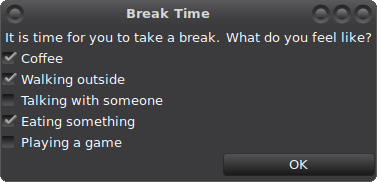
\includegraphics{images/mvp-screenshot.png}
  \caption{Client MVP}
  \label{fig:mvp-screenshot}
\end{figure}

\subsection{APIs}
% what technologies were chosen and why?
The basic APIs were designed among the first components during the development. The APIs development includes the definition of the communication protocol channels, models and the possible values that are sent between the client and the server in both directions. 

In terms of technology, a traditional RESTful \footnote{url{https://en.wikipedia.org/wiki/Representational\_state\_transfer}} API was chosen and designed. The chosen data format is JSON \footnote{\url{https://en.wikipedia.org/wiki/JSON}} due to its simplicity, easiness and wide usage in the present time. 

The APIs are not discussed further and are out of the scope of this document. Nevertheless, the history of the git repository and the model's source code is available via the GitHub page \footnote{url{https://github.com/InteractiveOfficeProject/api-documentation}} and the HTML documentation is made public via the department's websites \footnote{url{http://pivanics.users.cs.helsinki.fi/interactive-office-api-documentation/}}. 

\section{Conclusions}
\label{sec:conclusions}
\subsection{Results}
% what are the results and outcomes of the project? 
The needfinding phase of the project identified the main stakeholders of any kind of office environments. Employees, employers and visitors are among the main actors, who regularly visit and spend considerable amount of time in the office. Furthermore, cleaners and customers visit such environment occasionally with slightly different purposes. 

% what are the identified needs? 
The literature research, interviews and observation highlighted that a connective point for all stakeholders is the fact that activities performed in the office environment are work-related. These activities typically require good atmosphere, collaboration and proper tools in order to achieve efficiency. Several tools exist already which assist office workers to perform their work more efficiently, for example by automation of repetitive tasks. 

Collaboration is often a challenge for many companies due to cultural gaps or other interpersonal issues. Office workers may not know eachother very well with respect to professional background and personal interests, which generates obstacles for fluent collaboration. Therefore, there is a possibility to enhance collaboration by enhancing relationships of co-workers.

Well-being and comfort are another aspects in establishing a good office environment, which strongly contributes to efficient work hours as well. For instance, studies show that people who take regular breaks and alter between tasks during their work are more efficient and achieve more by the end of the day. However, we concluded trough observation and literature review that some workers resist to take breaks while performing their daily work. 

% what was the idea?
Our project put focus on to develop a tool, which enhances break habits and thereby improves social relationships and well-being of individuals working in office environments. This is done by tracking worker activity by for instance pressure sensors in their chair, keyboard activity or face recognition tracking through a web camera. Ultimately, the users could have some kind of sensors that track signals of the body (for instance pulse or heart rate) to determine how "aware" the person is. The scope of such development was excluded from the project, but could be interesting for further research. 

% what was developed? 
The basis of a software were developed, which can enhance break habits of office workers. Based on the Pomodoro technique, the software notifies the person after certain amount of work time (for example 25 minutes). The software suggests employees to take a break by picking an activity/topic and by finding a partner or multiple partners to spend the break with. Activities can be chosen from a list, which is retrieved from a remote database. 

By participating in different activities with colleagues, breaks become more interactive and fun. Workers stand up from their desk, socialize, experience something new around their regular working environment. Consequently, the motivation of workers to go on breaks increases, social relationships and collaboration among colleagues enhance. 

Matching up the partners for the break is completely random at this point of time. However, it would be interesting to gather data about the background and interests of the users and perform the matching based on the interests in common. Once the break is over, users return to their desk, fill the feedback form and continue to work. The feedback form investigates the overall feeling of the person after the break is over, how he/she feels, did he/she meet somebody new at the company or did he/she learn something new about the colleagues. 

\subsection{Evaluation}
In the final phases of the project, a brief heuristic/expert evaluation of the software was performed by the researchers. For this evaluation, the guidelines of Nielsen and Molich were used \cite{nielsen} \cite{nielsenonline}. 

We systematically analyzed the ten points of general principles of heuristic evaluation in regard to our software. The findings are listed below. 

\begin{enumerate}
	\item \textbf{Visibility of system status}: the system status is visible in the appearing windows, however may not be clear in some cases. For example, the main window of the application does not give any instructions in what state the application is or what the user should do. In case the user is in the queue/working status, the timer on top does not clearly tell that he/she has the given amount of time left, e.g. that the timer is a countdown. The rest of the windows are otherwise explaining the status well, but there is certainly room for improvements on the main window. 
	\item \textbf{Match between system and the real world}: the terminology used by the application is understandable as the targeted users understand the relationship of work and breaks. However, there is a lack of instructions around the application's views, which could greatly contribute to the understandability of the actions a user can perform.
	\item \textbf{User control and freedom}: there is quite a few functions which the application supports at the present time and which makes the possible user actions are fairly limited. Therefore this aspect is not the most important from the list. Nevertheless, the application does not allow to change the selection of the selected activities once they are chosen, which could be a good feature to add in regard to this heuristic. 
	\item \textbf{Consistency and standards}: the appearance of the current windows is aligned with the standards of the platform on which they were taken. Accordingly, there is no major need for further improvements in this regard. However, as more features are added, this aspect should be kept in mind.
	\item \textbf{Error prevention}: error prevention was already added on the windows, where there is a possibility to make an error. For instance, users cannot join the match queue without selecting at least one activity or match up with a person, without actually selecting one. 
	\item \textbf{Recognition rather than recall}: the number of features is limited, so is the number of visual objects that are open for interaction. Users would probably not have much problems recalling what individual buttons do as their placement, labeling and appearance tells their purpose clearly. However, the lack of instructions may be an issue for new users and therefore more instructions should be added to the screens.
	\item \textbf{Flexibility and efficiency of use}: accelerators and super users were not yet considered during the project and therefore this aspect is excluded from the analysis.
	\item \textbf{Aesthetic and minimalist design}: the aesthetics of the windows could be improved by slightly bigger windows and more legible text. The application currently is a bit "boring" and is lacking of joy in use. There is not any extra or irrelevant information on the screen either, but the current design may be "too minimalistic". 
	\item \textbf{Help users recognize, diagnose, and recover from errors}: the application could guide the users with some tips and hints in case an error over just graying out the buttons on the screen. 
	\item \textbf{Help and documentation}: there is room for improvement on both in-application help and documentation for the software as these were not considered in the current state of development in any ways. 
\end{enumerate}

\subsection{Future plans}
On top of the heuristic evaluation above, it would be interesting to see how users experience the software in a real environment. For example, it would be interesting direction for further research to observe how the atmosphere changes at a big corporate organization who uses this software. As the current state of the software is lacking some advanced functionality, pieces could be substituted for the study, for example by paper based or manual work. 

% what was not done and how the software could be improved?
A wide range of future development can be done on this project. Our future plans for the project include, but are not limited to 
\begin{enumerate}
	\item the detailed evaluation of the current software,
	\item experimenting with the software in a real environment,
	\item extension of the break-identification mechanism by
		\begin{enumerate}
			\item tracking keyboard activity of the user,
			\item tracking lifetime of a process on the users's computer,
			\item pressure-sensor integration to the users' chairs,
			\item analysis of body-signals to identify tiredness,
		\end{enumerate}
	\item matching algorithm for the users,
	\item automatic analysis of feedback data.
\end{enumerate}


\pagebreak
\nocite{*}
\bibliographystyle{tktl}
\bibliography{references}


\lastpage
\appendices
\pagestyle{empty}
\singlespacing

\internalappendix{1}{Break habits \& collaboration during work - Interview questions}
\label{sec:interview-questions}
Before asking the questions below to the interviewee, introduce your and the project?s background. Ask permission from the interviewee, if he/she has 10-15 minutes time to conduct the interview with you. Point out that the interviewee will remain anonymous. If you would like to record the session for further reference and analysis, make sure to ask permission.

\begin{enumerate}
\item Please introduce yourself shortly!
\item Tell me about your working field and environment! 
\item Do you think you take enough breaks during your work? 
\item Describe what do you do during your breaks! What do your breaks like? 
\item Do you interact with others during your breaks? 
\item Do you talk about work-related issues during your breaks? 
\item Do you know the professional skillset and hobbies of your colleagues well?
\item What is the standard way to in your organization to get to know the skillset of co-workers? 
\item Do you know whom to contact if you have work-related question? Are these people easy to reach? 
\item What do you do when you are stuck at work? 
\item What could be the reasons if collaboration between colleagues are not fluent/good? 
\end{enumerate}

\internalappendix{2}{Related Work}
\label{sec:related-work}
Studies in real working environments are hard to do: the situation cannot be controlled and the 
study must impact the working people as less as possible. To conduct research, a controlled 
environment is needed. Researchers at the university of Kaiserslautern created the living lab to 
merge these requirements. The living lab is an open space office that was designed with the goal to 
conduct research in the area of Smart Offices \cite{living-lab}.

The living lab has researched different types of technologies. Examples include electrochromatic 
glass which can be turned dark on demand to prevent sunlight from shining trough or personalized air 
flow optimization for workers. The living lab tests these technologies in simulations and real life 
situations. Another area of research is light and acoustic optimization. Good lighting and acoustics 
cannot be measured directly as most people only notice bad lighting or bad acoustics \cite{living-lab}.

\internalappendix{3}{Crowdboard invitation}
\begin{quote}
Hi Turkers,

we are three students working on a project for the course "Designing Interactive Systems" at University of Helsinki. The goal of our project to analyze working environments and develop ways to improve well-being and interaction. Part of our vision to reach this goal is to study break habits and facilitate employees towards more social interactions during their breaks. 

To improve on existing ideas and find new ideas, you are invited to join a live design session with our design team and help us to generate ideas. Time and invitation link are listed below.

Time: Thursday, 23rd March 2017, 14:30
Join link: (Insert Link to session here)

The Crowdboard is an augmented whiteboard which enables you to help us by adding input directly to the whiteboard - either by commenting on existing ideas or putting new ideas to the board - online, from your personal computer. Because the Crowdboard is still in development and too many comments/ideas would overwhelm us, there will be a limit of 20-30 people that can add comments. 

Thanks in advance,
Jan, Michael, Péter
\end{quote}

\internalappendix{4}{Crowdboard initial task}
\begin{quote}
We are three students working on a project for the course "Designing Interactive Systems" at University of Helsinki. The goal of our project to analyze working environments and develop ways to improve well-being and interaction. Part of our vision to reach this goal is to study break habits and facilitate employees towards more social interactions during their breaks. 

Your task is help us analyzing the break habits of employees in an office environment and to generate ideas in what ways breaks can lead to better interaction, well-being and collaboration of co-workers. Welcome! 
\end{quote}

\internalappendix{5}{Screenshots from the application}
	\begin{center}
		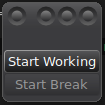
\includegraphics{images/app-screenshots/mainwindow-cropped.png} \\
		
		The main window of the application. The user enter start the working phase by pressing on Start Working. 
		
		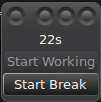
\includegraphics{images/app-screenshots/working-cropped.png} \\
		
		The window for the "working" phase. The timer on the top indicates for how long the user has been working for. By pressing on Start Break, the user enters the "in break" phase and the activity selection window is displayed. 
	
		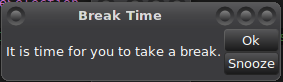
\includegraphics{images/app-screenshots/break-notification-cropped.png} \\
		
		The break notification which appears when the system recognizes the need for a break. The user has the possibility to Snooze the notification or accept the break invitation by pressing Ok. 
		
		\pagebreak
		
		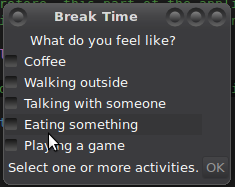
\includegraphics{images/app-screenshots/activity-selection.png} \\
		
		The activity selection window after the user has accepted the invitation for the break. The users can select one or more acitivites from the list for which a partner or multiple partners will be found. 
		
		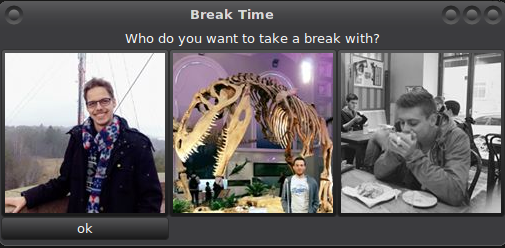
\includegraphics[width=1\textwidth]{images/app-screenshots/people-selection-cropped.png} \\
		
		The people selection window, which appears after partners for the breaks have been found. By pressing on any of the appearing user profile pictures the break between two people are started.
	\end{center}
	

\end{document}
